% Architecture of the dense decoder-only model built in post 7 (Qwen3-0.6B shape).
% Visual language of Figure 1 of "Attention Is All You Need": narrow boxes sized to
% their text, thick black outlines, large labels, grey rounded container for the
% repeat. Annotations are spelled out in words rather than symbols, so the figure
% reads on its own without the surrounding post.
%
% Vertical layout: every box is ~1.6cm tall, so centres are spaced ~2.3 apart to
% leave a visible ~0.8 arrow between them. Branch points for the residual paths sit
% midway between a box edge and the next, never on an edge.
%
% Build:
%   tectonic model-architecture.tex           (or: pdflatex model-architecture.tex)
%   pdftoppm -png -r 300 model-architecture.pdf model-architecture
%   mv model-architecture-1.png model-architecture.png

\documentclass[border=16pt]{standalone}
\usepackage{tikz}
\usepackage{helvet}
\renewcommand{\familydefault}{\sfdefault}
\usetikzlibrary{arrows.meta,backgrounds,decorations.pathreplacing}

% Palette taken from the original paper figure.
\definecolor{cEmbed}{RGB}{250,214,214}   % pink   - embedding / LM head (tied)
\definecolor{cAttn} {RGB}{252,222,182}   % orange - attention
\definecolor{cFFN}  {RGB}{196,224,247}   % blue   - feed-forward
\definecolor{cNorm} {RGB}{240,240,186}   % yellow - normalization
\definecolor{cSoft} {RGB}{198,231,200}   % green  - softmax
\definecolor{cBlock}{RGB}{239,239,239}   % grey   - repeated block container

\begin{document}
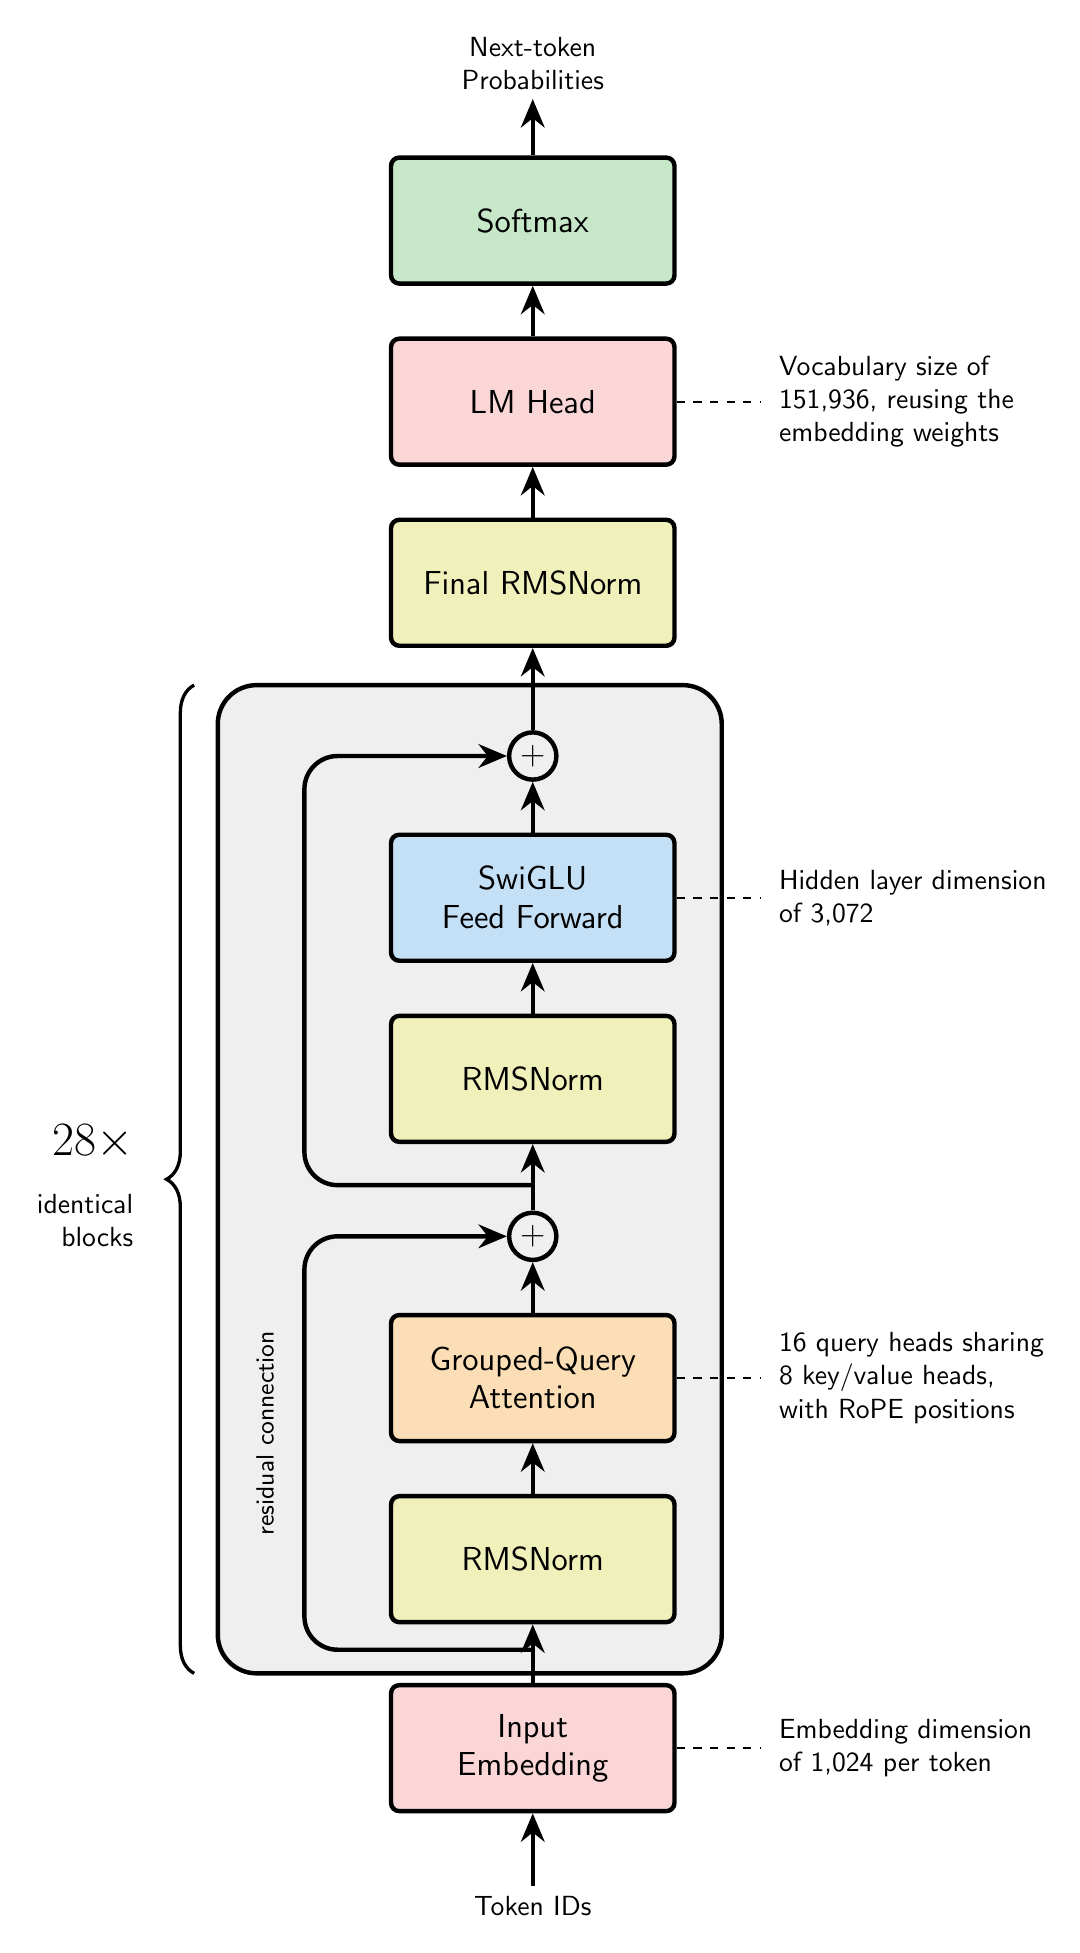
\begin{tikzpicture}[
  >={Stealth[length=3.6mm,width=3mm]},
  % uniform minimum height so single-line and two-line boxes match
  blk/.style={draw,line width=1.6pt,rounded corners=3pt,
              minimum width=3.6cm,minimum height=1.6cm,
              align=center,inner sep=6pt,font=\large},
  op/.style={draw,circle,line width=1.6pt,minimum size=0.6cm,inner sep=0pt,font=\large},
  arr/.style={->,line width=1.6pt},
  note/.style={font=\normalsize,align=left,inner sep=2pt},
  edge/.style={font=\normalsize,align=center},
  lead/.style={line width=0.7pt,dashed},
]

% ------------------------------------------------------------------ main column
\node[edge]            (in)   at (0,-0.2) {Token IDs};
\node[blk,fill=cEmbed] (emb)  at (0,1.8)  {Input\\Embedding};
\node[blk,fill=cNorm]  (n1)   at (0,4.2)  {RMSNorm};
\node[blk,fill=cAttn]  (att)  at (0,6.5)  {Grouped-Query\\Attention};
\node[op]              (a1)   at (0,8.3)  {$+$};
\node[blk,fill=cNorm]  (n2)   at (0,10.3) {RMSNorm};
\node[blk,fill=cFFN]   (ffn)  at (0,12.6) {SwiGLU\\Feed Forward};
\node[op]              (a2)   at (0,14.4) {$+$};
\node[blk,fill=cNorm]  (nf)   at (0,16.6) {Final RMSNorm};
\node[blk,fill=cEmbed] (head) at (0,18.9) {LM Head};
\node[blk,fill=cSoft]  (sm)   at (0,21.2) {Softmax};
\node[edge]            (out)  at (0,23.2) {Next-token\\Probabilities};

% ------------------------------------------------- repeated block (grey container)
\begin{scope}[on background layer]
  \draw[rounded corners=14pt,line width=1.6pt,fill=cBlock]
        (-4.0,2.75) rectangle (2.4,15.3);
\end{scope}

% brace + repeat count on the left, so it is read before the block it labels
\draw[line width=1.2pt,decorate,decoration={brace,amplitude=10pt}]
      (-4.3,2.75) -- (-4.3,15.3);
\node[font=\LARGE,anchor=east]            at (-4.95,9.5) {$28\times$};
\node[font=\normalsize,anchor=east,align=right] at (-4.95,8.5) {identical\\blocks};

% ------------------------------------------------------------------- main flow
\draw[arr] (in)   -- (emb);
\draw[arr] (emb)  -- (n1);
\draw[arr] (n1)   -- (att);
\draw[arr] (att)  -- (a1);
\draw[arr] (a1)   -- (n2);
\draw[arr] (n2)   -- (ffn);
\draw[arr] (ffn)  -- (a2);
\draw[arr] (a2)   -- (nf);
\draw[arr] (nf)   -- (head);
\draw[arr] (head) -- (sm);
\draw[arr] (sm)   -- (out);

% -------------------------------------------------- residual bypasses (pre-norm)
% The stream is never normalized: it branches off below each RMSNorm and rejoins
% at the plus, so the norm sits on the branch rather than on the stream.
\draw[arr,rounded corners=12pt]
      (0,3.05) -- (-2.9,3.05) -- (-2.9,8.3) -- (a1);
\draw[arr,rounded corners=12pt]
      (0,8.95) -- (-2.9,8.95) -- (-2.9,14.4) -- (a2);
\node[font=\small,rotate=90] at (-3.4,5.8) {residual connection};

% ------------------------ annotations, written out in words rather than symbols
\draw[lead] (emb.east)  -- (2.9,1.8);
\node[note,anchor=west] at (3.05,1.8)  {Embedding dimension\\of 1,024 per token};

\draw[lead] (att.east)  -- (2.9,6.5);
\node[note,anchor=west] at (3.05,6.5)  {16 query heads sharing\\8 key/value heads,\\with RoPE positions};

\draw[lead] (ffn.east)  -- (2.9,12.6);
\node[note,anchor=west] at (3.05,12.6) {Hidden layer dimension\\of 3,072};

\draw[lead] (head.east) -- (2.9,18.9);
\node[note,anchor=west] at (3.05,18.9) {Vocabulary size of\\151,936, reusing the\\embedding weights};

\end{tikzpicture}
\end{document}
